\documentclass{beamer} 
\setbeamertemplate{navigation symbols}{}

\usepackage{beamerthemeshadow}
\usepackage[utf8]{inputenc}
\usepackage[magyar]{babel}
\usepackage[T1]{fontenc}
\usepackage{amsmath}
\usepackage{amsfonts}
\usepackage{amssymb}
\usepackage{graphicx}
\usepackage{lmodern}
\usepackage{textcomp}
\usepackage{listings}
\usepackage{xcolor}
\usepackage{textcomp}
\usepackage{mathtools}
\usepackage{epsfig}

\author{Haraszti Gábor \\DPWF3Y}
\title{Diplomamunka 2}
\subtitle{beszámoló prezentáció}
\date{\today}

\begin{document} 

\begin{frame} 
\titlepage
\end{frame}

\begin{frame} 
\frametitle{Elvégzett munka összefoglalása}
\begin{itemize}
\item Bevezetés,
\item Irodalmi áttekintés,
\item Felhasznált technológiák bemutatása,
\item A megvalósítandó rendszer specifikációja
\end{itemize}
\end{frame}

\begin{frame} 
\frametitle{Bevezetés}
\begin{itemize}
	\item Felhő technológiák megjelenésének hatása a robotikára,
	\item Keletkezett adatmennyiség 80\% nem ember által létrehozott,
	\item Szolgáltató és ipari robotok közötti különbség, ISO
	13482-es szabvány szerint:
	\begin{description}
	\item[ipari robot:] Az ipari robot egy automatikus irányítású, újraprogramozható, többcélú automatikus ipari feladatok elvégzésére használt manipulátor, három vagy több tengelye programozható, melyek lehetnek rögzítettek vagy mobilak.
	\item[szolgáltató:] Olyan robot, amely hasznos feladatokat hajt végre emberek vagy berendezések számára, kivéve az ipari automatizáló berendezéseket.
	\end{description}
\end{itemize}
\end{frame}

\begin{frame} 
\frametitle{Irodalmi áttekintés}
\begin{itemize}
	\item 8 publikáció feldolgozása,
	\item Konténer technológia tanulmányozása,
	\item Robot Operating System tanulmányozása,
	\item Felhő technológiák, Rapyuta,
\end{itemize}
\end{frame}

\begin{frame} 
\frametitle{Felhasznált technológiák bemutatása}
\begin{itemize}
	\item Operációs rendszer kiválasztása: Ubuntu 16.04 LTS,
	\item Virtualizációs technológia, Docker konténer,
	\item Felhő szolgáltatók bemutatása,
	\item ROS bemutatása
\end{itemize}
\end{frame}

\begin{frame} 
\frametitle{Docker kapcsolata a Linux kernellel}
	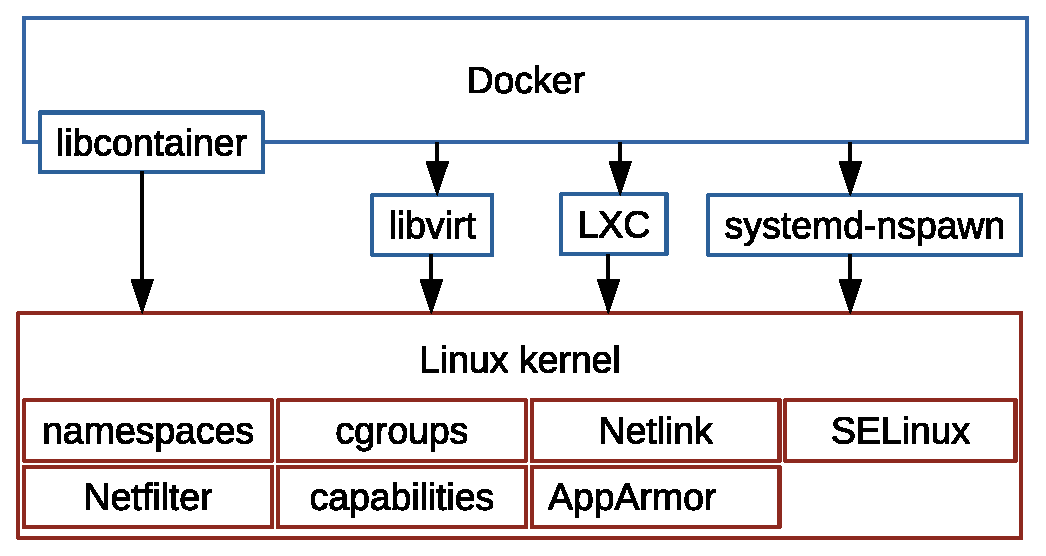
\includegraphics[width=11cm]{../docker-architektura}
\end{frame}

\begin{frame} 
\frametitle{ROS Architektúra}
	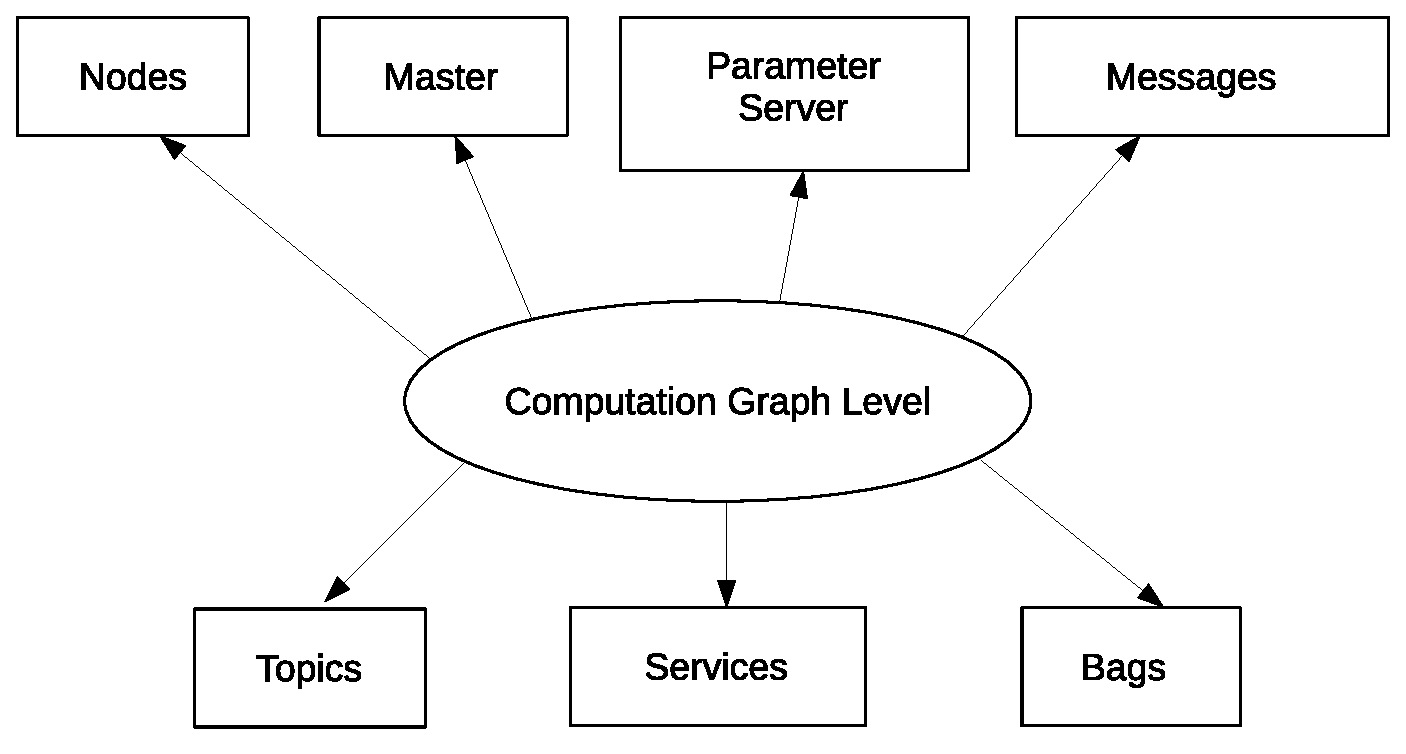
\includegraphics[width=11cm]{../ROS}
\end{frame}

\begin{frame} 
\frametitle{A megvalósítandó rendszer specifikációja}
\begin{itemize}
	\item Proof of Concept,
	\item Minta feladat: pályatervezés,
	\item Felhő és lokális megvalósítás,
	\item Docker, Rosbridge, Cloudroid használata
\end{itemize}
\end{frame}

\begin{frame} 
\frametitle{Docker - ROS konfiguráció}
	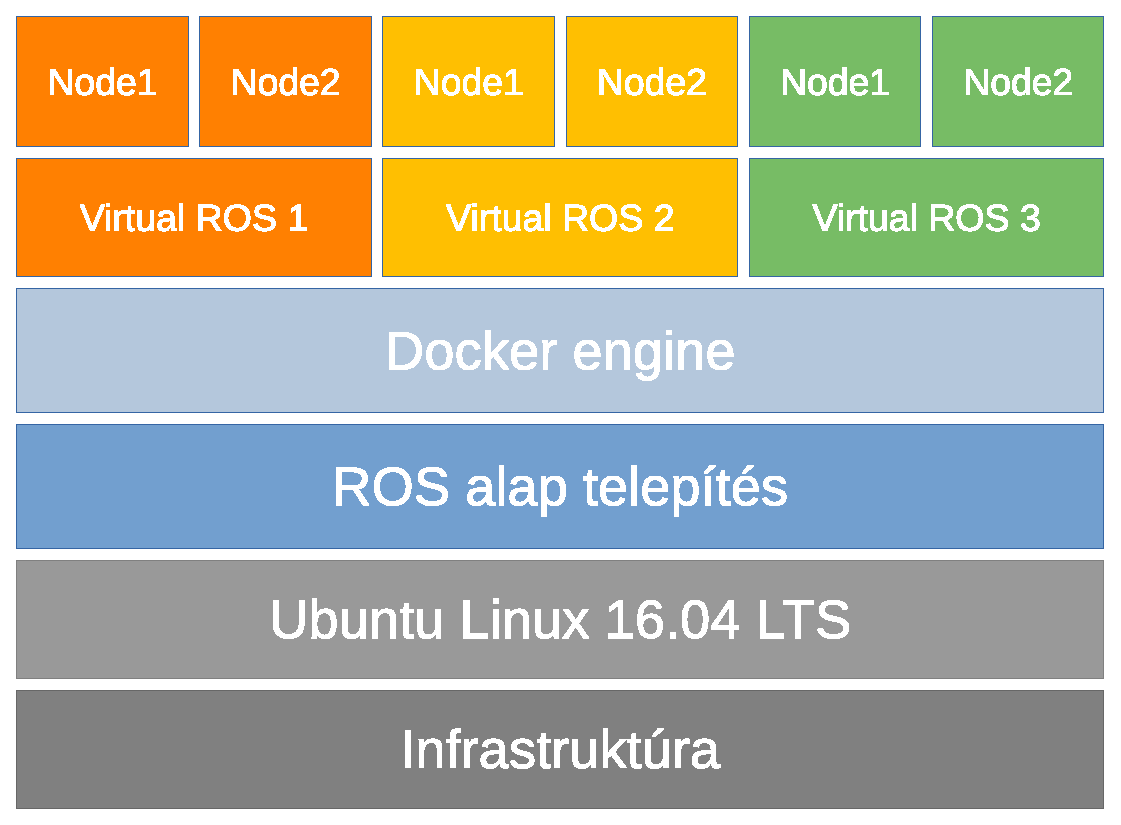
\includegraphics[width=11cm]{../feladat-architektura-ROS}
\end{frame}

\begin{frame} 
\frametitle{Felhő konfiguráció}
	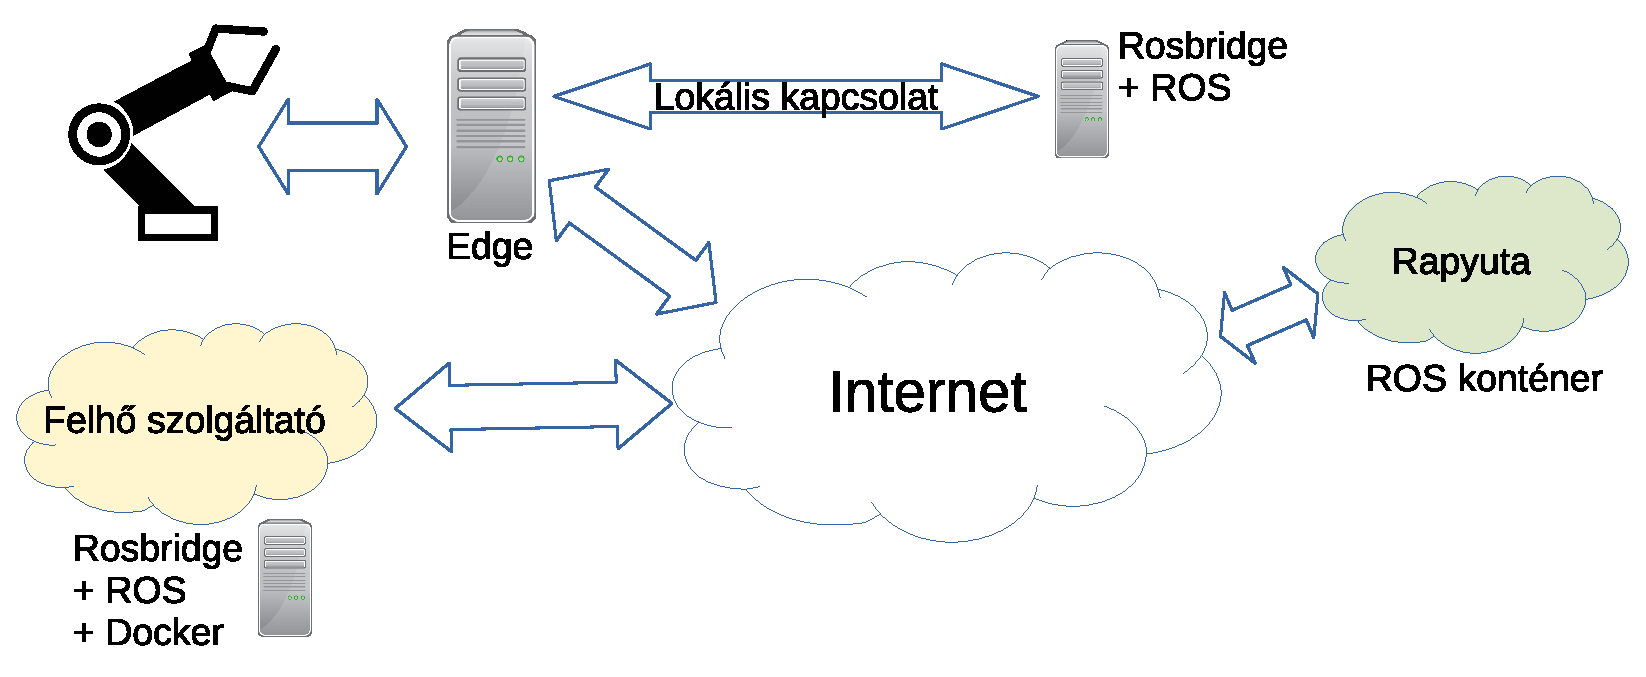
\includegraphics[width=11cm]{../docker-architektura-Felho}
\end{frame}


\begin{frame} 
\frametitle{Vége}
\begin{center}
	{\Huge Köszönöm a figyelmet!}
\end{center}
\end{frame}

\end{document}	